\documentclass[11pt]{article}
\usepackage[utf8]{inputenc}
\usepackage[spanish]{babel}

% Paquetes

\usepackage{amsmath}
\usepackage{amsthm}
\usepackage{amsfonts}
\usepackage{amssymb}
\usepackage{makeidx}
\usepackage{graphicx}
\usepackage{lmodern}
%\usepackage{kpfonts}
\usepackage{fancyhdr}
\usepackage{geometry}
\usepackage{lastpage}
\usepackage{fancybox} % para usar la caja de los ejemplos
\usepackage[font=small, justification=centering]{caption}  % Configura las captions
\usepackage{multirow}
\usepackage{longtable} % para tablas largas
\usepackage{xcolor}
\usepackage{listings}
\usepackage{tikz}
\usepackage{subcaption}
%##############################################################################
%######### Formato lstlisting #################################################
%##############################################################################


\definecolor{codegreen}{rgb}{0,0.6,0}
\definecolor{codegray}{rgb}{0.5,0.5,0.5}
\definecolor{codepurple}{rgb}{0.58,0,0.82}
\definecolor{backcolour}{rgb}{0.95,0.95,0.92}



\lstdefinestyle{mystyle}{
    backgroundcolor=\color{backcolour},   
    commentstyle=\color{codegreen},
    keywordstyle=\color{magenta},
    numberstyle=\tiny\color{codegray},
    stringstyle=\color{codepurple},
    basicstyle=\ttfamily\footnotesize,
    breakatwhitespace=false,         
    breaklines=true,                 
    captionpos=b,                    
    keepspaces=true,                 
    numbers=left,                    
    numbersep=5pt,                  
    showspaces=false,                
    showstringspaces=false,
    showtabs=false,                  
    tabsize=2
}

\lstset{style=mystyle}


%##############################################################################
%######### Geometría #################################################
%##############################################################################

\geometry{a4paper, total={152mm,237mm}, left=31mm, top=32mm}

%##############################################################################
%######### Formatos capítulo #################################################
%##############################################################################

%\usepackage[lmodern]{quotchap}
%\usepackage[options]{fncychap}

%##############################################################################
%######### Hiperreferenias #################################################
%##############################################################################
\usepackage[colorlinks=true,allcolors=blue]{hyperref} % Crea las


%##############################################################################
%######### Formato de pagina #################################################
%##############################################################################

\renewcommand{\sectionmark}[1]{\markright{\thesection.\ #1}}

\setlength{\headsep}{27pt} % Distancia entre la cabezera y el texto
\setlength{\footskip}{25pt} % Distancia entre el pie de pagina y el texto
\pagestyle{fancy}
\fancyhf{}
\fancyhead[LE,RO]{Creación de la configuración inicial} % L,R,C-> left, right, center [LE,RO]% E,O -> even (par), odd (impar)
\fancyhead[LO,RE]{Daniel Vázquez Lago}
\fancyfoot[CE,CO]{\thepage}
\renewcommand{\headrulewidth}{1pt} % Cambiamos el grosor de la linea de arriba
\renewcommand{\footrulewidth}{0pt}


% Autor y título
\author{Daniel Vazquez Lago}
\title{Memoria 1 Simulación en física de Materiales}

\newcommand{\rn}{\mathbf{r}}
\newcommand{\vn}{\mathbf{v}}
\newcommand{\Fn}{\mathbf{F}}
\newcommand{\an}{\mathbf{a}}

\newcommand{\parentesis}[1]{\left( #1  \right)}
\newcommand{\parciales}[2]{\frac{\partial #1}{\partial #2}}
\newcommand{\pparciales}[2]{\parentesis{\parciales{#1}{#2}}}
\newcommand{\ccorchetes}[1]{\left[ #1  \right]}
\newcommand{\D}{\mathrm{d}}
\newcommand{\derivadas}[2]{\frac{\D #1}{\D #2}}


\begin{document}


\maketitle
\newpage

\tableofcontents


\section{Objetivos}

El objetivo de esta primera entrega de la asignatura es generar un sistema de 500 partículas con una densidad de 0.5 y energía E=575 (variables reducidas), que en posteriores entregas se usará como base para crear una simulación donde las partículas se muevan e interaccionen entre ellas, esto es, se usará como base para hacer una simulación de dinámica molecular. Consecuentemente esta simulación tendrá que dar un valor a las siguientes variables:

\begin{itemize}
	\item La posición de las 500 partículas.
	\item La velocidad/momento de las 500 partículas.
	\item La aceleración/fuerza de las 500 partículas.
	\item La energía cinética ($T$) y potencial ($V$) del sistema, verificando que $T+V=575$.
	\item La derivada primera y segunda de la energía potencial respecto el volumen (que usaremos para calcular valores como la presión, el coeficiente de comprensibilidad...).
\end{itemize}
Además de crear el sistema, también se nos pide que guardemos los datos más relevantes de esta configuración inicial en un archivo \texttt{.dat}. 

\section{Procedimiento} \label{Sec:02}

En el proyecto ajunto se puede ver que el orden para definir las variables es el siguiente: 

\begin{enumerate}
	\item Posiciones de las 500 partículas.
	\item Energía potencial, sus derivadas respecto al volumen del sistema y las aceleraciones de las partículas. 
	\item Velocidades de las partículas y energía cinética
\end{enumerate}
Mientras que el último paso será guardar todos los datos en un archivo. Uno podría pensar que este orden es gratuito, pero nada mas lejos de la realidad, este orden es el correcto para generar la configuración inicial, tal y como veremos a continuación. \\

En los siguientes apartados se describirá como se han definido las variables y porqué lo hemos hecho así, todo desde un punto de vista puramente teórico, dejando la programación para la sección \ref{Sec:03}.


\subsection{Posiciones de las partículas}

En esta práctica las partículas se han colocado disponiendo una red fcc, de tal manera que nuestro sistema será una caja (cubo) formado por un número determinado de celdas convencionales (que tienen, por definición, el mismo volumen y el mismo número de partículas encerradas en su interior). \\

La razón por la cual se ha elegido una configuración fcc tiene que ver con la energía potencial. Una red fcc nos permite colocar las partículas a una distancia lo suficientemente grande como para que, inicialmente, la interacción entre estas partículas sea débil. De colocar las partículas con una variable aleatoria correríamos el riesgo de que dos partículas estuvieran lo suficientemente cerca como para que la interacción entre ellas las llevara a tener una energía potencial (y por ende una aceleración) tan elevada que podría producir un error a la hora de realizar la dinámica molecular. \\

Veamos como definir adecuadamente una red fcc. Dado que el sistema cúbico total debe estar formado por un número $n$ entero de celdas convencionales, no es difícil darse cuenta que $n$ viene dado por $k^3$ donde $k\in\mathbb{Z^+}$ \footnote{Para esto basta con ver que el lado del sistema $L$ debe estar compuesto por un número entero de lados pequeños (si no uno se ``saldría'') tal que si $L=nl$, debe verificarse que $V=n^3V_{\textbf{celda}}$}. Y como cada celda convencional del sistema fcc contiene 4 puntos de red (4 partículas) el número de partículas debe verificar que $N=4k^3$, esto es: $N\in\{4,32,108,256,500,864...\}$. Nosotros elegimos un $k=5$ y por tanto un número de partículas $N=500$. \\

La colocación de las partículas se hará entonces de la siguiente manera: colocamos 4 partículas por cada una de las celdas convencionales, recorriendo con un lazo triple las 125 celdas convencionales. Cada celda convencional colocará las partículas según la siguiente imagen:

\begin{figure}[h!]	\centering		
\begin{tikzpicture}[scale=3]
	
	% Dibujar los vértices del cubo
	
	% Etiquetas de los ejes
	%	\draw[->] (-0.2,0,0) -- (1.3,0,0) node[anchor=north east] {$x$};
	%	\draw[->] (0,-0.2,0) -- (0,1.3,0) node[anchor=north west] {$y$};
	%	\draw[->] (0,0,-0.2) -- (0,0,1.3) node[anchor=south] {$z$};
	
	% Aristas del cubo
	\draw[thick] (0,0,0) -- (1,0,0);
	\draw[thick] (0,0,0) -- (0,1,0);
	\draw[thick] (0,0,0) -- (0,0,1);
	\draw[thick] (1,0,0) -- (1,1,0);
	\draw[thick] (1,0,0) -- (1,0,1);
	\draw[thick] (0,1,0) -- (1,1,0);
	\draw[thick] (0,1,0) -- (0,1,1);
	\draw[thick] (0,0,1) -- (1,0,1);
	\draw[thick] (0,0,1) -- (0,1,1);
	\draw[thick] (1,1,0) -- (1,1,1);
	\draw[thick] (1,0,1) -- (1,1,1);
	\draw[thick] (0,1,1) -- (1,1,1);
	
	% Dibujar los átomos en el centro de las caras
	\filldraw[red] (0,0,1) circle (0.07); % Esquina
	\filldraw[red] (0.5,0.5,1) circle (0.07); % Cara xy abajo
	\filldraw[red] (0.5,0,0.5) circle (0.07); % Cara xz izquierda
	\filldraw[red] (0,0.5,0.5) circle (0.07); % Cara yz delante
	
	% Relaciones entre puntos
	
	\draw[thick] (0,0,0.5) -- (0,0.5,0.5);
	\draw[thick] (0,0.5,1) -- (0,0.5,0.5);	
	
	\draw[thick] (0,0,0.5) -- (0.5,0,0.5);
	\draw[thick] (0.5,0,1) -- (0.5,0,0.5);
	
	\draw[thick] (0.5,0,1) -- (0.5,0.5,1);
	\draw[thick] (0,0.5,1) -- (0.5,0.5,1);
	
	
\end{tikzpicture}
\caption{Colocación de las 4 partículas en una celda convencional.}
\end{figure}

Como podemos ver en la siguiente imagen, las celdas convencionales colocarán las 500 partículas en un sistema fcc perfectamente:

\begin{figure}[h!]	\centering		
	\begin{tikzpicture}[scale=2]
		
		% Dibujar los vértices del cubo
		\foreach \x in {0,1,2,3,4} {
			\foreach \y in {0,1,2,3,4} {
				\foreach \z in {0} {
					\draw[thick] (\x,\y,\z) -- (1+\x,\y,\z);
					\draw[thick] (\x,\y,\z) -- (\x,1+\y,\z);
					\draw[thick] (\x,\y,\z) -- (\x,\y,1+\z);
					\draw[thick] (1+\x,\y,\z) -- (1+\x,1+\y,\z);
					\draw[thick] (1+\x,\y,\z) -- (1+\x,\y,1+\z);
					\draw[thick] (\x,1+\y,\z) -- (1+\x,1+\y,\z);
					\draw[thick] (\x,1+\y,\z) -- (\x,1+\y,1+\z);
					\draw[thick] (\x,\y,1+\z) -- (1+\x,\y,1+\z);
					\draw[thick] (\x,\y,1+\z) -- (\x,1+\y,1+\z);
					\draw[thick] (1+\x,1+\y,\z) -- (1+\x,1+\y,1+\z);
					\draw[thick] (1+\x,\y,1+\z) -- (1+\x,1+\y,1+\z);
					\draw[thick] (\x,1+\y,1+\z) -- (1+\x,1+\y,1+\z);
					
					% Dibujar los átomos en el centro de las caras
					\filldraw[red] (\x,\y,\z+1) circle (0.07); % Esquina
					\filldraw[red] (\x+0.5,0.5+\y,1+\z) circle (0.07); % Cara xy abajo
					\filldraw[red] (0.5+\x,0+\y,0.5+\z) circle (0.07); % Cara xz izquierda
					\filldraw[red] (0+\x,0.5+\y,0.5+\z) circle (0.07); % Cara yz delante
					
					% Relaciones entre puntos
					
					\draw[thick] (0+\x,0+\y,0.5+\z) -- (0+\x,0.5+\y,0.5+\z);
					\draw[thick] (0+\x,0.5+\y,1+\z) -- (0+\x,0.5+\y,0.5+\z);	
					
					\draw[thick] (0+\x,0+\y,0.5+\z) -- (0.5+\x,0+\y,0.5+\z);
					\draw[thick] (0.5+\x,0+\y,1+\z) -- (0.5+\x,0+\y,0.5+\z);
					
					\draw[thick] (0.5+\x,0+\y,1+\z) -- (0.5+\x,0.5+\y,1+\z);
					\draw[thick] (0+\x,0.5+\y,1+\z) -- (0.5+\x,0.5+\y,1+\z);
				}
			}
		}
	\end{tikzpicture}
	\caption{Colocación de las celdas convencionales.}
\end{figure}

Sin embargo la colocación mostrada tiene un problema, y es que la alta simetría de la disposición puede crear comportamientos raros para la posterior dinámica molecular, por lo que lo resolveremos dándole una pequeña ``sacudida''. En otras palabras, vamos a sumarle/restarle un valor aleatorio suficientemente pequeño como para no generar el problema de que dos partículas muy juntas, pero suficientemente alto como para que no sea perfectamente simétrico. Si cada celda convencional tiene un lado de tamaño $a=L/5$ (recordemos que si $N=500$ y $\rho=0.5$, $V=N/\rho=1000$ y $L=10$), la sacudida debería de ser entorno a un 10\% la mitad del lado de la celda convencional. Podríamos aumentar esta sacudida hasta un 15\% o incluso un 20\%, de tal manera que el sistema sería cada vez menos simétrico y por tanto mucho mas cercano a una posición del gas natural, pero con esto nos arriesgaremos a que haya problemas con la energía. Un 10\% es más que suficiente.

\subsection{Condiciones de contorno periódicas}


La frontera de la caja donde tenemos encerradas las partículas es un problema, ya que no podemos exigir que se mantenga la densidad constante sin exigir al sistema alguna condición de contorno, como por ejemplo que las partículas estén encerradas, de tal manera que colisionen elásticamente con la pared. Sin embargo, nosotros queremos simular un gas libre de 500 partículas, y al exigir esto los resultados obtenidos serían de otro tipo de simulación \cite{Haile}. \\

La mejor manera de evitar estes choques con la superficie, es imponer las condiciones de contorno periódicas. La condición de contorno periódica parte de algo muy interesante que es considerar nuestra caja de 500 partículas es una parte representativa (\textit{celda primaria}) de un gas infinito constituido por nuestra celda repetida infinitas veces por todo el espacio. De esta forma, cada vez que salga una partícula por un lado, llegará por el lado contrario otra partícula, con la misma velocidad (no hay pérdida de información). Así el número de partículas en la celda es constante. Esto se ve claramente en la siguiente imagen (ejemplo en 2D):

\begin{figure}[h!]	\centering		
	\begin{tikzpicture}[scale=2.1]
		
		% Dibujar los vértices del cubo
		\foreach \x in {0,1,2} {
			\foreach \y in {0,1,2} {
				\draw[thick] (\x,\y) -- (\x+1,\y);
				\draw[thick] (\x,\y) -- (\x,\y+1);
				\draw[thick] (\x+1,\y+1) -- (\x,\y+1);
				\draw[thick] (\x+1,\y) -- (\x+1,\y+1);				
			}
		}
		\foreach \x in {0,1,2} {
			\foreach \y in {0,1,2} {			
				\filldraw[red] (\x,0.5+\y) circle (0.07);
				\filldraw[red] (\x+1,0.5+\y) circle (0.07); % Cara yz delante			
				\draw[thick] (\x,0.5+\y) -- (\x+0.25,0.5+\y);
				\draw[thick] (\x+1,0.5+\y) -- (\x+1.25,0.5+\y);	
				
				\draw[thick] (\x+0.25,0.5+\y) -- (\x+0.2,0.45+\y);
				\draw[thick] (\x+0.25,0.5+\y) -- (\x+0.2,0.55+\y);
				\draw[thick] (\x+1.25,0.5+\y) -- (\x+1.2,0.45+\y);	
				\draw[thick] (\x+1.25,0.5+\y) -- (\x+1.2,0.55+\y);	
			}
		}	
		
		\node at (1.5,1.1) {{\tiny Celda primaria}};
	\end{tikzpicture}
	\caption{Cuando una partícula entra, otra sale.}
\end{figure}

A pesar de todo, esta condición nos va a obligar a exigir un radio máximo para la interacción de dos partículas, ya que una partícula no puede interactuar dos veces con la misma partícula en sentidos opuestos, ya que esto alteraría la interacción y tendríamos una simulación errónea. Debemos imponer que la distancia máxima para la que puede haber interacción será $L/2$, y la llamaremos \textit{radio de corte} $r_c$ (con los datos presentados antes tenemos $r_c=5$). La siguiente imagen muestra el efecto:

\begin{figure}[h!]	\centering		
	\begin{subfigure}{0.45\linewidth} \centering
	\begin{tikzpicture}[scale=2]
		
		% Dibujar los vértices del cubo
		\foreach \x in {0,1,2} {
			\foreach \y in {0,1,2} {
				\draw[thick] (\x,\y) -- (\x+1,\y);
				\draw[thick] (\x,\y) -- (\x,\y+1);
				\draw[thick] (\x+1,\y+1) -- (\x,\y+1);
				\draw[thick] (\x+1,\y) -- (\x+1,\y+1);				
			}
		}
		\foreach \x in {0,1,2} {
			\foreach \y in {0,1,2} {			
				\filldraw[red,opacity=0.8] (\x+0.4,\y+0.4) circle (0.03);
				\filldraw[red,opacity=0.8] (\x+0.2,\y+0.1) circle (0.03);
				\filldraw[red,opacity=0.8] (\x+0.69,\y+0.7) circle (0.03);
				\filldraw[red,opacity=0.8] (\x+0.59,\y+0.1) circle (0.03);
				\filldraw[red,opacity=0.8] (\x+0.29,\y+0.73) circle (0.03);
				\filldraw[red,opacity=0.8] (\x+0.91,\y+0.15) circle (0.03);
				\filldraw[red,opacity=0.8] (\x+0.05,\y+0.93) circle (0.03);
				\filldraw[red,opacity=0.8] (\x+0.02,\y+0.43) circle (0.03);
				\filldraw[red,opacity=0.8] (\x+0.92,\y+0.89) circle (0.03);
		}	
		
		\filldraw[blue] (1.4,1.4) circle (0.03);
		delante			
		\draw[blue] (1.4,1.4) circle(0.5);
		}
		
	\end{tikzpicture}
	\caption{Solo interacciona con una partícula $r_c=L/2$.}
	\end{subfigure}
	\begin{subfigure}{0.45\linewidth} \centering
	\begin{tikzpicture}[scale=2]
		
		% Dibujar los vértices del cubo
		\foreach \x in {0,1,2} {
			\foreach \y in {0,1,2} {
				\draw[thick] (\x,\y) -- (\x+1,\y);
				\draw[thick] (\x,\y) -- (\x,\y+1);
				\draw[thick] (\x+1,\y+1) -- (\x,\y+1);
				\draw[thick] (\x+1,\y) -- (\x+1,\y+1);				
			}
		}
		\foreach \x in {0,1,2} {
			\foreach \y in {0,1,2} {			
				\filldraw[red,opacity=0.8] (\x+0.4,\y+0.4) circle (0.03);
				\filldraw[red,opacity=0.8] (\x+0.2,\y+0.1) circle (0.03);
				\filldraw[red,opacity=0.8] (\x+0.69,\y+0.7) circle (0.03);
				\filldraw[red,opacity=0.8] (\x+0.59,\y+0.1) circle (0.03);
				\filldraw[red,opacity=0.8] (\x+0.29,\y+0.73) circle (0.03);
				\filldraw[red,opacity=0.8] (\x+0.91,\y+0.15) circle (0.03);
				\filldraw[red,opacity=0.8] (\x+0.05,\y+0.93) circle (0.03);
				\filldraw[red,opacity=0.8] (\x+0.02,\y+0.43) circle (0.03);
				\filldraw[red,opacity=0.8] (\x+0.92,\y+0.89) circle (0.03);
			}	
		}
			\filldraw[blue] (1.4,1.4) circle (0.03);
			delante			
		\draw[blue] (1.4,1.4) circle(0.59);
			
		\foreach \x in {0,1} {
			\foreach \y in {1} {
				\filldraw[green,opacity=0.8] (\x+0.91,\y+0.15) circle (0.03);
			}
		}	
		
	\end{tikzpicture}
	\caption{Interacciona con dos partículas análogas $r_c>L/2$.}
	\end{subfigure}
\end{figure}


\subsection{Energía potencial}

Hemos hablado en los dos apartados de la interacción de las partículas así como de la energía potencial, pero sin llegar a definirla, y tampoco decir para que la necesitamos. El potencial o energía potencial es una manera de describir la interacción de dos partículas. En nuestro caso el potencial entre ambas solo dependerá de la posición de estas $v_{ij} = v(\rn_i,\rn_j)$ ($i,j$ partículas cualquiera tal que $i\neq j$). Nosotros usaremos el \textbf{potencial Lennard-Jones}, que viene dado por la ecuación (variables reducidas)

\begin{eqnarray}
	v_{ij} = 4 \ccorchetes{\parentesis{\frac{1}{r_{ij}}}^{12}-\parentesis{\frac{1}{r_{ij}}}^6}
\end{eqnarray}

\begin{figure}[h!] \centering
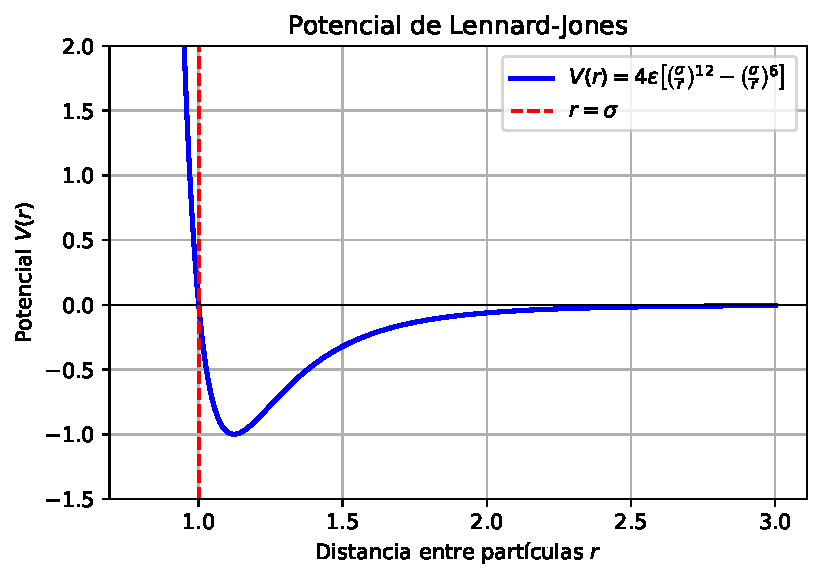
\includegraphics[scale=0.95]{Lennard-jones.pdf}
\caption{Potencial de Lennard-jones para variables reducidas ($\epsilon,\sigma = 1$)}
\end{figure}    
Esto es, las partículas a cortas distancias se repelen, mientras que a grandes distancias se atraen débilmente. En general este tipo de potenciales describe bien a gases con baja interacción (como los gases nobles) parecidos a los gases ideales, por lo que es perfecta para un primer acercamiento a la dinámica molecular. También podemos ver que cuando $r \rightarrow \infty$ la interacción tiende a cero (así como su primera y segunda derivada respecto $r$), y por tanto imponer un radio de corte $r_c=L/2=5$ no alterará mucho la dinámica de cada partícula, por lo que será una buena aproximación (no hay apenas de continuidad y derivabilidad). En cualquier caso, corregiremos el error producido por el potencial generado para $r>5$, no tanto por que sea un problema en este ejercicio en particular, si no porque produciría un error sistemático, que se acumulará en cada interacción, y teniendo en cuenta que haremos 5 millones de interacciones (como mínimo), supondrá un problema en la dinámica molecular. \\

\subsubsection{Correción de la energía}


La forma de corregir esta interacción es sencilla, ya que podemos recurrir a ciertas aproximaciones, como vamos a ver a continuación. En general la energía potencial $E_p$ viene dada por:

\begin{eqnarray}
	\frac{E_p}{N} =  2\pi \rho \int_0^\infty g(r) v(r) r^2 \D r 
\end{eqnarray}
donde $g(r)$ es la función de distribución radial y $v(r)$ el potencial. En este caso nosotros ya estamos teniendo en cuenta la energía potencial de $0$ a $r_c$ ($\langle E_p \rangle$), lo que queremos saber es la correción por no tener en cuenta los radios $r>r_c$. Dado que podemos hacer:

\begin{eqnarray*}
	\frac{E_p}{N} =  2\pi \rho \int_0^{r_c} g(r) v(r) r^2 \D r + 2\pi \rho \int_{r_c}^\infty g(r) v(r) r^2 \D r  
\end{eqnarray*}
esto nos lleva a que

\begin{eqnarray}
	\frac{E_p}{N} =  \frac{\langle E_p \rangle}{N} + 2\pi \rho \int_0^{r_c} g(r) v(r) r^2 \D r + 2\pi \rho \int_{r_c}^\infty g(r) v(r) r^2 \D r  
\end{eqnarray}
Y por tanto la \textit{correción de la energía por partícula} es

\begin{eqnarray}
	u_{LR} = 2\pi \rho  \int_{r_c}^\infty  g(r) v(r) r^2 \D r  
\end{eqnarray}
Dado que estamos estudiando un gas casi ideal con un radio de corte razonablemente grande se verificará que $g(r)=1$, de tal modo que la integral  

\begin{eqnarray}
	u_{LR} = 2\pi \rho  \int_{r_c}^\infty \ccorchetes{\parentesis{\frac{1}{r}}^{10}-\parentesis{\frac{1}{r}}^4}  \D r  
\end{eqnarray}
La integral es trivial, por lo que escribimos directamente que

\begin{eqnarray}
	u_{LR} = 2 \pi \rho \parentesis{\frac{1}{3} \frac{1}{r_c^3} - \frac{1}{9} \frac{1}{r_c^9}} = \frac{2\pi \rho}{3 r_c^3} \parentesis{1-\frac{1}{3} \frac{1}{r_c^6}} \approx \frac{2\pi \rho}{3 r_c^3}  
\end{eqnarray}
Así la \textit{energía total} tendrá un valor real de

\begin{eqnarray}
	E_p=  \langle E_p \rangle + N \frac{2\pi \rho}{3 r_c^3}  
\end{eqnarray}
aunque en los cálculos usaremos la aproximación completa.

\subsubsection{Derivadas del potencial}

La energía potencial y su primera y segunda derivadas respecto el volumen ($\langle \varphi_V \rangle$ y $\langle \varphi_{VV} \rangle$ respectivamente) son términos fundamentales para calcular posteriormente factores como la presión, la capacidad calorífica, entre otras. Por tanto es necesario obtener sus valores, los cuales se deducen a partir de 

\begin{equation}
	v_{ij}' (r_{ij}) = \derivadas{v_{ij}}{r_{ij}} = -24 \ccorchetes{2\frac{1}{r_{ij}^{13}}- \frac{1}{r_{ij}^7}} = -\frac{24}{r_{ij}} \ccorchetes{2\frac{1}{r_{ij}^{12}} - \frac{1}{r_{ij}^6}} 
\end{equation}	
\begin{equation}
	v_{ij}''(r_{ij}) = \frac{\D^2v_{ij}}{(\D r_{ij})^2} = 24 \ccorchetes{13\frac{1}{r_{ij}^{14}}- 7\frac{1}{r_{ij}^8}} = \frac{24}{r_{ij}^2} \ccorchetes{26\frac{1}{r_{ij}^{12}}- 7\frac{1}{r_{ij}^6}} \\ 
\end{equation}
tal que si el potencial $\varphi(\rn) = \sum_{i=1}^{N-1} \sum_{j=i}^N v_{ij} (r_{ij})$, relacionamos 


\begin{equation}
	\langle \varphi_V \rangle = \sum_{i=1}^{N-1}\sum_{j=i+1}^{N} \parciales{v_{ij} (r_{ij})}{r_{ij}} \parciales{r_{ij}}{L} \parciales{L}{V}
\end{equation}
lo que nos lleva a que:

\begin{equation}
	\langle \varphi_V \rangle = \frac{1}{3V} \sum_{i=1}^{N-1}\sum_{j=i+1}^{N}  r_{ij} v_{ij}'(r_{ij})
\end{equation}
La segunda derivada:


\begin{equation}
	\langle \varphi_{VV} \rangle =\parciales{}{V} \parentesis{\frac{1}{3V} \sum_{i=1}^{N-1}\sum_{j=i+1}^{N}  r_{ij} v_{ij}'(r_{ij})}
\end{equation}
nos lleva a que

\begin{equation}
	\langle \varphi_{VV} \rangle = \frac{1}{3V} \ccorchetes{\frac{1}{3V} \sum_{i=1}^{N-1} \sum_{i=i+1}^{N} r_{ij}^2 v_{ij}''(r_{ij})	- 2 \parentesis{\parciales{\varphi}{V}}}
\end{equation}
En cualquier caso debemos tener en cuenta que estamos sumando sobre todas las partículas pero hemos limitado por las condiciones de contorno que $v_{ij}=0$ si $r_{ij}>r_c$. Entonces estas también tendrán una correción parecida a la que hemos hecho en la energía. De esta forma tenemos que 

\begin{eqnarray}
	\varphi_{V} = \langle \varphi_V \rangle  + \frac{16\pi N^2}{3V r_c^3} \parentesis{-\frac{2}{3 r_c^6}+1}
\end{eqnarray}
\begin{eqnarray}
	\varphi_{VV} = \langle \varphi_V \rangle  + \frac{16\pi N^2}{3V r_c^3} \parentesis{-\frac{26}{3 r_c^6}-7}
\end{eqnarray}

\subsubsection{Cálculo de la fuerza}

Una vez tenemos esto calcular la fuerza es un ejercicio casi trivial. Basta con ver que la fuerza ejercida sobre una partícula $k$ viene dada por:

\begin{eqnarray}
	\Fn_{k} = - \derivadas{E_p}{\rn_k}
\end{eqnarray}
y que por tanto (realmente aquí se han hecho pasos no tan triviales, pero dado que está deducido en el Tema 3, obviamos algunos de ellos):

\begin{eqnarray}
	\Fn_{k} =\frac{1}{2}  \sum_{j\neq k}^N v_{kj}' \frac{\rn_{kj}}{r_{kj}}
\end{eqnarray}
Si definimos el término $F_{kj}^{mod}$ como

\begin{eqnarray}
	F_{kj}^{mod} =- \frac{v_{kj}'}{r_{kj}} = \frac{24}{r_{kj}^2} \ccorchetes{2 \parentesis{\frac{1}{r_{kj}}}^{12}-\parentesis{\frac{1}{r_{kj}}}^6}
\end{eqnarray}
tenemos que 

\begin{eqnarray}
	\Fn_{k} = \sum_{j \neq k} F_{kj}^{mod} \rn_{kj}
\end{eqnarray}
Dado que $F_{kj}^{mod}=F_{jk}^{mod}$, y que $\rn_{kj}=-\rn_{jk}$, es evidente que $\sum_{k=1}^N \Fn_k=0$. Para nosotros, como tenemos tenemos un hamiltoniano normal, las aceleraciones verifican $\an_k = \Fn_k$, aunque hay que tener cuidado.


\subsection{Velocidades y energía cinética}

Para dar una velocidad a nuestro sistema bastará con asignar un valor aleatorio entre -1 y 1 a cada componente de la velocidad de cada una de las partículas, de tal manera que no conozcamos con precisión el valor real de la velocidad. Sin embargo tenemos que exigir dos cosas a nuestras velocidades: que el momento total sea nulo y que $\sum_i v_i^2/2 = T$. Que el momento total sea nulo es una exigencia plausible, ya que estamos estudiando un gas estático. Además esta condición nos permite minimizar los errores. En principio aplicar la corrección es sencilla, basta con calcular la velocidad total del sistema en un eje (tengamos por ejemplo el $x$, aunque se haga de manera análoga en el $y$ y en el $z$) $v_{x}^T = \sum_{i=1}^N v_{xi}$, de tal modo que la nueva velocidad de la partícula $i$ sobre el eje $x$ será la anterior menos la total entre el número de partículas $v_{xi}^{\text{nueva}}=v_{xi}^{\text{vieja}}-v_x^T/N$. \\

Dado que en este punto ya conocemos la energía potencial del sistema $E_p$, y que la energía total $E=575$ ya está definida, la energía cinética $T$ tiene un valor único:

\begin{eqnarray}
	T=E-E_p
\end{eqnarray}
Entonces debemos modificar de alguna forma el módulo de nuestras velocidades para que se verifique que, efectivamente $\sum_i v_i^2/2 = T$. Para esto basta con normalizar las velocidades, lo que implica dividir por $v=\sqrt{(v_x^T)^2+(v_y^T)^2+(v_z^T)^2}$ cada una de las componentes y multiplicar cada una de ellas por $\sqrt{2\cdot T}$. 
	 
\section{Simulación} \label{Sec:03}

Con todo lo visto antes comprender cada paso que damos ahora, de tal manera que no nos detendremos a comentar cada paso con tanta intensidad como antes. En esta sección nos limitaremos a describir un poco como está organizado el proyecto y que podemos encontrar en él. 

\subsection{Módulos}

\subsubsection{Módulo 1: define precisión}

\subsubsection{Módulo 2: variables comunes}

\subsubsection{Módulo 3: interface}


\subsection{Programa principal}

Descripción de las variables: \\

Código:

\subsection{Subrutina energía potencial}

Descripción de las variables: \\

Código:

\bibliography{Bibliografia.bib}
\bibliographystyle{unsrt}


\end{document}
